%\documentclass[10pt,aspectratio=169]{beamer}
\documentclass[10pt]{beamer}

\usetheme[progressbar=frametitle]{metropolis}
\usepackage{appendixnumberbeamer}

\usepackage{booktabs}
\usepackage[scale=2]{ccicons}

\usepackage{pgfplots}
\usepgfplotslibrary{dateplot}

\usepackage{biblatex} 


\usepackage{xspace}
\newcommand{\themename}{\textbf{\textsc{metropolis}}\xspace}

\newcommand\blfootnote[1]{%
	\begingroup
	\renewcommand\thefootnote{}\footnote{#1}%
	\addtocounter{footnote}{-1}%
	\endgroup
}

\title{Sicherheit in der IT-Infrastruktur}
\subtitle{Beispiele aus der Praxis, Ausfallsicherheit, Backups, Verschlüsselung}
% \date{\today}
\date{14.03.2019}
\author{Timo Schindler}
\institute{OTH Regensburg}
% \titlegraphic{\hfill\includegraphics[height=1.5cm]{logo.pdf}}

\begin{document}

\maketitle

%%%%%%%%%%
%
% Inhalt
%
%%%%%%%%%%
\begin{frame}{Inhalt}
  \setbeamertemplate{section in toc}[sections numbered]
  \tableofcontents[hideallsubsections]
\end{frame}

\section{Einführung: Backup}

%%%%%%%%%%
%
% Über mich
%
%%%%%%%%%%
\begin{frame}[fragile]{Über Mich}

\begin{columns}[T,c,onlytextwidth]
\column{0.5\textwidth}
\begin{exampleblock}{Timo Schindler}
OTH Regensburg
\end{exampleblock}

\column{0.5\textwidth}
\begin{itemize}
  	\item Promotion: IT Security \& Machine Learning
  	\item Server- und Storage-Systeme
  	\item Virtualisierungs-Infrastruktur
  	\item Sysadmin mit Leidenschaft
\end{itemize}
\end{columns}
\end{frame}


%%%%%%%%%%
%
% Zentralisierung als Lösung
%
%%%%%%%%%%
\begin{frame}[fragile]{Zentralisierung als Lösung?}
\begin{columns}[T,c,onlytextwidth]
	\column{0.5\textwidth}
	\begin{itemize}
		\item In Zeiten von Cloud: Services wandern in die Rechenzentren
		\item Zentraler Zugriff für alle Benutzer
		\item Zentraler Schwachpunkt
		\item Vertrauen in Administratoren
		\item Sicherheit an Zentraler Stelle wichtiger den je!
	\end{itemize}

\column{0.5\textwidth}
 \begin{figure}
	
\includegraphics[width=0.8\textwidth]{images/thereisnocloud-v2}
\end{figure}
\end{columns}
	\blfootnote{Bild: \href{https://fsfe.org/activities/nocloud}{https://fsfe.org/activities/nocloud}}
\end{frame}

%%%%%%%%%%
%
% Warum Backup?
%
%%%%%%%%%%
\begin{frame}[fragile]{Warum Backup?}
Gründe für Backups sehr divers. Datenverlust durch:
	\begin{itemize}
	\item Versehentliches Löschen
	\item Unberechtigte Veränderung durch Dritte
	\item Technischer Systemausfall
	\item Diebstahl, Sabotage, Betrug
	\item Katastrophen (Brand, Wasserschaden)
	\item Angriffe (z.B. Ransomware)
\end{itemize}
Backupmechanismen und -maßnahmen unterscheiden sich dadurch erheblich.
\end{frame}

%%%%%%%%%%
%
% Schutzziele der Informationssicherheit
%
%%%%%%%%%%
\begin{frame}[fragile]{Schutzziele der Informationssicherheit}
\begin{columns}[T,onlytextwidth]
	\column{0.45\textwidth}
	Allgemeine Schutzziele
	
	\metroset{block=fill}
	\begin{exampleblock}{Vertraulichkeit}
		Lesen nur durch autorisierte Benutzer
	\end{exampleblock}
	
	\begin{exampleblock}{Integrität}
		Keine unbemerkte Veränderung
	\end{exampleblock}
	
	\begin{exampleblock}{Verfügbarkeit}
		Verhinderung von Systemausfällen
	\end{exampleblock}
	
	\column{0.45\textwidth}
	Weiter Schutzziele
	
	\metroset{block=fill}
	\begin{exampleblock}{Authentizität}
		Echtheit bzw. Überprüfbarkeit eines Objektes
	\end{exampleblock}
	
	\begin{exampleblock}{Verbindlichkeit}
		Kein unzulässiges Abstreiten von Aktionen
	\end{exampleblock}
	
	\begin{exampleblock}{Zurechenbarkeit}
		Zuordnung einer Aktion auf Benutzer
	\end{exampleblock}
	
\end{columns}

Schutzziele können nur durch Zusammenspiel aus Hard- und Software erreicht werden.
\end{frame}

%%%%%%%%%%
%
% Maßstab für Ausfallsicherheit
%
%%%%%%%%%%
\begin{frame}[fragile]{Maßstab für Ausfallsicherheit}
\begin{alertblock}{Tier 1 - Die Holzklasse}
\end{alertblock}
		\begin{columns}[T,c,onlytextwidth]
		\column{0.6\textwidth}
			\begin{itemize}
			\item Keine Redundanz
			\item Jährliche Ausfallzeit 28,8 Stunden
			\item 99,67 \% Verfügbarkeit
			\item Wartung im Betrieb nicht möglich
			\item Nur ein Versorgungsweg für Kälte- und Energieverteilung
		\end{itemize}
		\column{0.4\textwidth}
	 \begin{figure}
		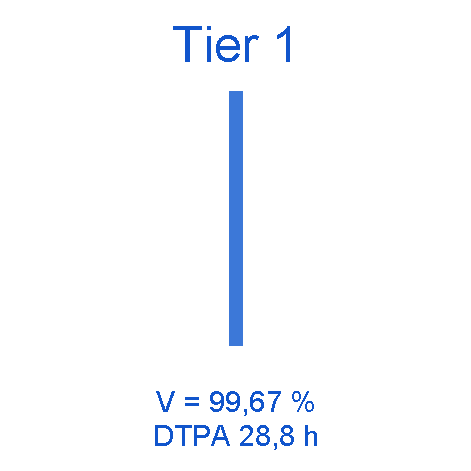
\includegraphics[width=1\textwidth]{images/tier1}
	\end{figure}
\end{columns}
\end{frame}

\begin{frame}[fragile]{Maßstab für Ausfallsicherheit}
\begin{alertblock}{Tier 2 - Einfache Redundanz im Rechenzentrum}
\end{alertblock}
\begin{columns}[T,c,onlytextwidth]
	\column{0.6\textwidth}
	\begin{itemize}
		\item Redundanz nur in Versorgungsweg
		\item Jährliche Ausfallzeit 22 Stunden
		\item 99,75 \% Verfügbarkeit
		\item Wartung im Betrieb bedingt möglich
		\item Redundanter Versorgungsweg für Kälte- und Energieverteilung
	\end{itemize}
	\column{0.4\textwidth}
	\begin{figure}
		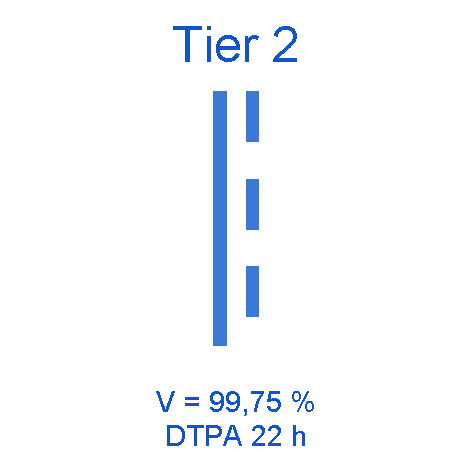
\includegraphics[width=1\textwidth]{images/tier2}
	\end{figure}
\end{columns}
\end{frame}

\begin{frame}[fragile]{Maßstab für Ausfallsicherheit}
\begin{alertblock}{Tier 3 - Fehlertoleranz möglich}
\end{alertblock}
\begin{columns}[T,c,onlytextwidth]
	\column{0.6\textwidth}
	\begin{itemize}
		\item Redundanz in Versorgung
		\item Server mehrfach vorhanden
		\item Jährliche Ausfallzeit 1,6 Stunden
		\item 99,98 \% Verfügbarkeit
		\item Wartung im Betrieb möglich
		\item Redundanter Versorgungsweg für Kälte- und Energieverteilung
	\end{itemize}
	\column{0.4\textwidth}
	\begin{figure}
		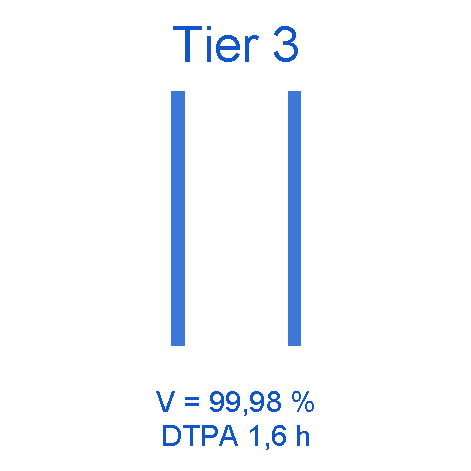
\includegraphics[width=1\textwidth]{images/tier3}
	\end{figure}
\end{columns}
\end{frame}

\begin{frame}[fragile]{Maßstab für Ausfallsicherheit}
\begin{alertblock}{Tier 4 - Die Masterclass}
\end{alertblock}
\begin{columns}[T,c,onlytextwidth]
	\column{0.6\textwidth}
	\begin{itemize}
		\item Komplette doppelte Redundanz
		\item Server mehrfach vorhanden
		\item Jährliche Ausfallzeit 0,8 Stunden
		\item 99,991 \% Verfügbarkeit
		\item Wartung im Betrieb möglich
		\item Mehrfach redundanter Versorgungsweg für Kälte- und Energieverteilung
	\end{itemize}
	\column{0.4\textwidth}
	\begin{figure}
		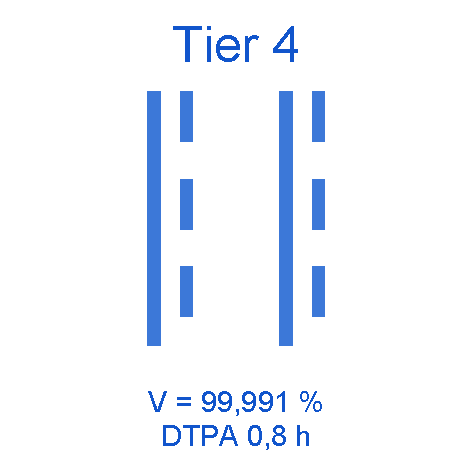
\includegraphics[width=1\textwidth]{images/tier4}
	\end{figure}
\end{columns}
\end{frame}

%%%%%%%%%%
%
% RAID
%
%%%%%%%%%%
\begin{frame}[fragile]{RAID ist kein Backup!}
\begin{columns}[T,c,onlytextwidth]
	\column{0.6\textwidth}
	\begin{itemize}
		\item Daten werden auf mehrere Festplatten verteilt
		\item Relative Ausfallsicherheit von Festplatten
		\item Problem bei Systematischen Fehlern
		\item Problem bei bestimmten RAID-Leveln
		\item RAID ist unverzichtbar, aber kein Backup!
	\end{itemize}
	\column{0.4\textwidth}
	\begin{figure}
		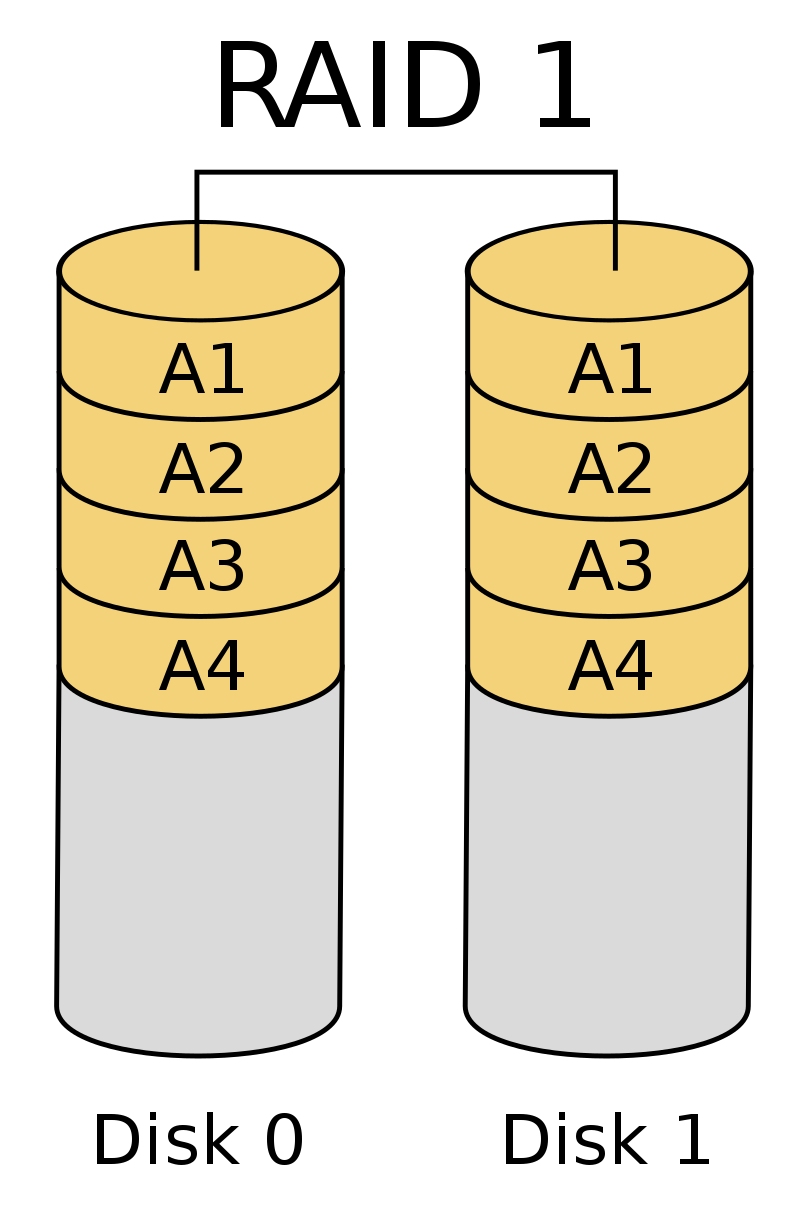
\includegraphics[width=1\textwidth]{images/RAID_1}
	\end{figure}
\end{columns}
	\blfootnote{Bild: \href{https://de.wikipedia.org/wiki/RAID}{https://de.wikipedia.org/wiki/RAID}}
\end{frame}

%%%%%%%%%%
%
% RAID 6
%
%%%%%%%%%%
\begin{frame}[fragile]{RAID ja, aber welche Konfiguration?}
\begin{alertblock}{RAID 6 oder 60}
\end{alertblock}
\begin{columns}[T,c,onlytextwidth]
	\column{0.6\textwidth}
	\begin{itemize}
		\item Bis zu zwei Festplatten können ausfallen
		\item Bei der Wiederherstellung von Festplatten oft Ausfall weiterer Platte
		\item Gutes Preis/Leistungs-Verhältnis
	\end{itemize}
	\column{0.4\textwidth}
	\begin{figure}
		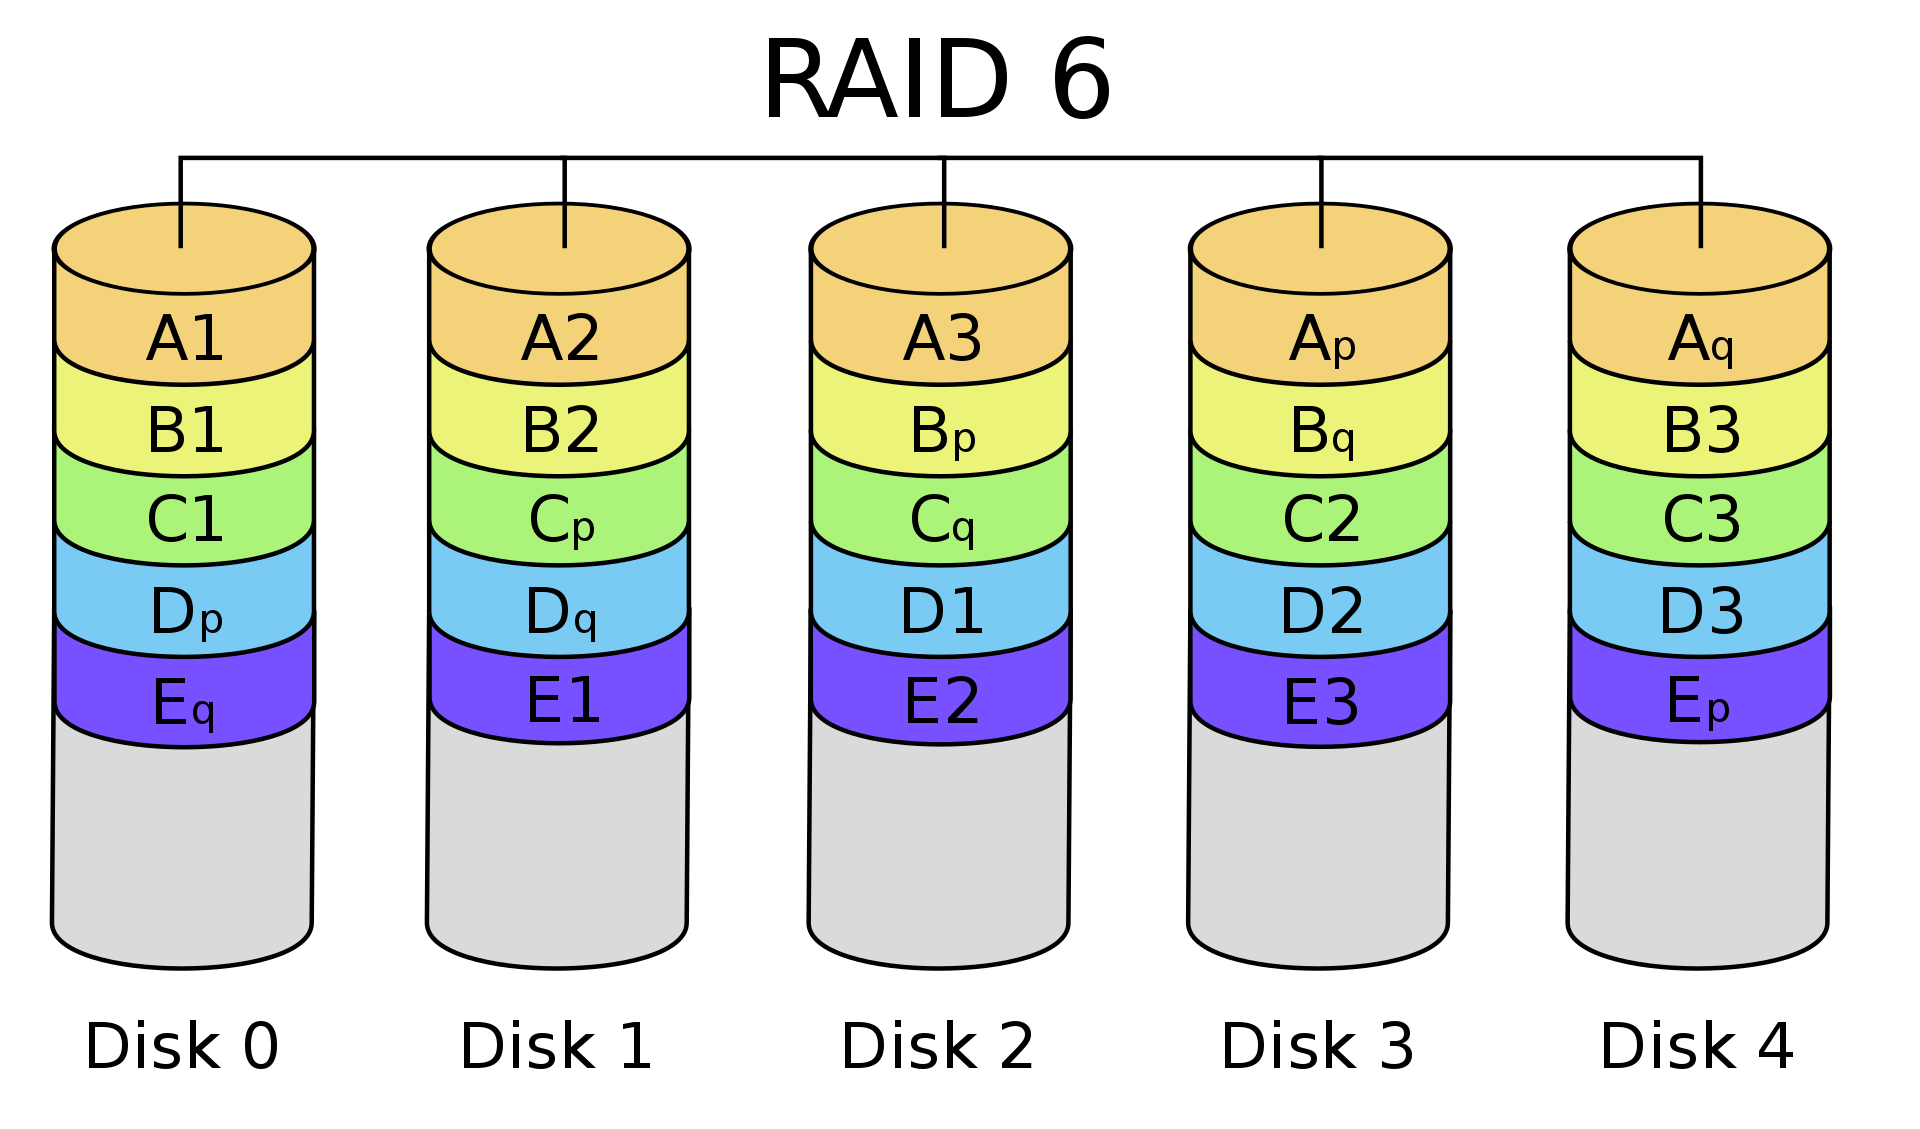
\includegraphics[width=1\textwidth]{images/RAID_6}
	\end{figure}
\end{columns}
	\blfootnote{Bild: \href{https://de.wikipedia.org/wiki/RAID}{https://de.wikipedia.org/wiki/RAID}}
\end{frame}

%%%%%%%%%%
%
% RAID Z2
%
%%%%%%%%%%
\begin{frame}[fragile]{Noch besser: RAID Z2}
\begin{alertblock}{Zettabyte File System}
\end{alertblock}
\begin{columns}[T,c,onlytextwidth]
	\column{0.6\textwidth}
\begin{itemize}
	\item Spezielles Filesystem
	\item Als Software-RAID umgesetzt
	\item Ausfallsicherheit wie RAID 6
	\item Reparatur von Files durch Hashes
	\item Möglich: Deduplizierung \& Kompression
	\item Möglich: Verschlüsselung \& Caching
\end{itemize}
	\column{0.4\textwidth}
	\begin{figure}
		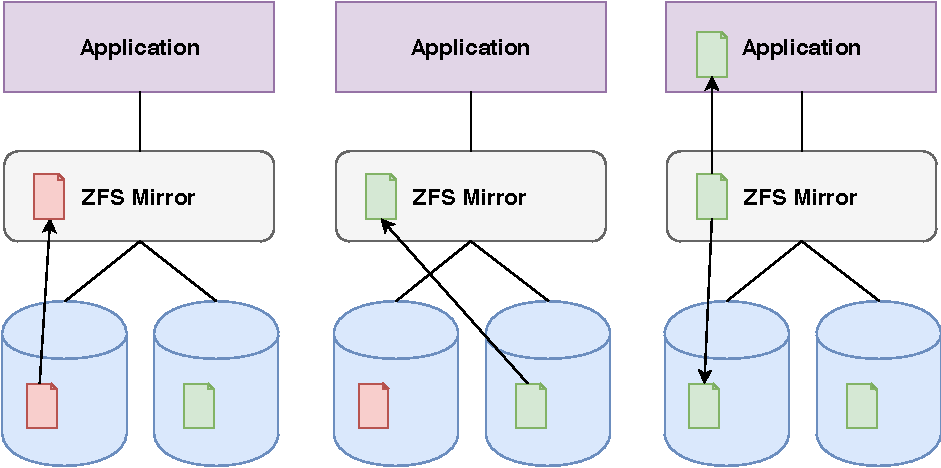
\includegraphics[width=1\textwidth]{images/zfs-self-healing}
	\end{figure}
\end{columns}
\end{frame}

%%%%%%%%%%
%
% Signaturen und Hashing Algorithmen
%
%%%%%%%%%%
\begin{frame}[fragile]{Signaturen und Hashing Algorithmen}
\begin{columns}[T,c,onlytextwidth]
	\column{0.6\textwidth}
	\begin{itemize}
		\item Einwegfunktion
		\item Hash immer gleiche Größe
		\item Gleiche Datei erzeugt gleichen Hash
		\item Minimale Änderungen erzeugen völlig unterschiedlichen Hash
		\item Kryptographische Sicherheit
	\end{itemize}
	\column{0.4\textwidth}
	\begin{figure}
		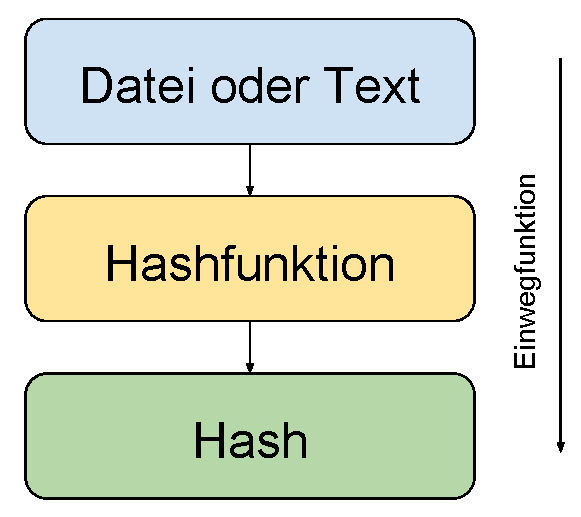
\includegraphics[width=1\textwidth]{images/hashing}
	\end{figure}
\end{columns}
\end{frame}

%%%%%%%%%%
%
% Spezialfall: Revisionssichere Archivierung
%
%%%%%%%%%%
\begin{frame}[fragile]{Spezialfall: Revisionssichere Archivierung}
	\begin{itemize}
	\item Schutz vor Manipulation
	\item Schutz vor nachträglicher Änderung
	\item Wird oft durch kryptografische Signaturen sichergestellt
	\item Zertifizierte Systeme sehr teuer
	\item Nötig für Compliance, Finanz- und Gesundheitsdaten
\end{itemize}
\end{frame}

%%%%%%%%%%
%
% Verschlüsselung
%
%%%%%%%%%%
\begin{frame}[fragile]{Verschlüsselung}
	\begin{itemize}
	\item Backups: Beliebtes Ziel für Datenmanipulation und -diebstahl
	\item Backups: Oft nachlässige Sicherheit
	\item Verschlüsselung macht Backup unbequem
	\item Eigener Infrastruktur sollte nicht vertraut werden
	\item Transportverschlüsselung nicht vergessen
\end{itemize}
\end{frame}

%%%%%%%%%%
%
% Vertraue keinem Backup!
%
%%%%%%%%%%
\begin{frame}[fragile]{Vertraue keinem Backup!}
\begin{alertblock}{Niemals!}
\end{alertblock}
\begin{columns}[T,c,onlytextwidth]
	\column{0.6\textwidth}
	\begin{itemize}
		\item Backups prüfen
		\item Ernstfall simulieren
		\item Mehrstufige Backups
		\item Nochmal Backups prüfen!
	\end{itemize}
	\column{0.4\textwidth}
	\begin{figure}
		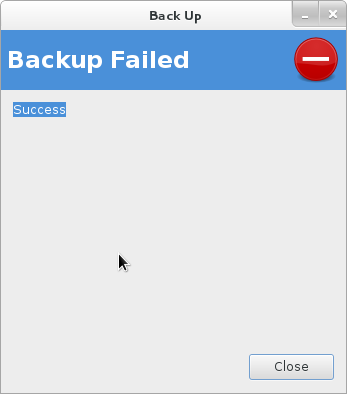
\includegraphics[width=1\textwidth]{images/failed-backup}
	\end{figure}
\end{columns}

\blfootnote{Bild: \href{https://mail.gnome.org/archives/deja-dup-list/2012-November/}{https://mail.gnome.org/archives/deja-dup-list/2012-November}}
\end{frame}

%%%%%%%%%%
%
% Notfallplan
%
%%%%%%%%%%
\begin{frame}[fragile]{Notfallplan}
\begin{columns}[T,c,onlytextwidth]
	\column{0.6\textwidth}
	\begin{itemize}
		\item Ausfälle passieren...
		\item ...zu unmöglichsten Zeiten
		\item Notfallplan aufstellen
		\item Infrastruktur funktioniert nicht
		\item Dauer?
		\item Ist diese Zeit vertretbar?
	\end{itemize}
	\column{0.4\textwidth}
	\begin{figure}
		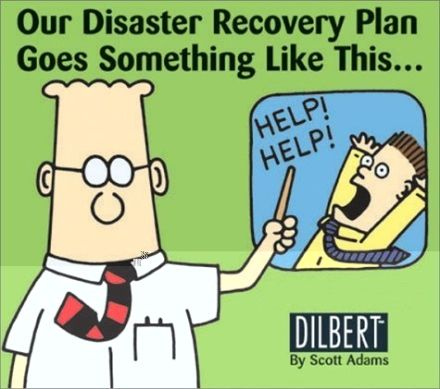
\includegraphics[width=1\textwidth]{images/dilbert}
	\end{figure}
\end{columns}

\blfootnote{Bild: \href{https://www.dilbert.com}{www.dilbert.com}}
\end{frame}

\section{Backupinfrastruktur in der Praxis}

%%%%%%%%%%
%
% Struktur OTH Regensburg
%
%%%%%%%%%%
\begin{frame}[fragile]{Struktur der OTH Regensburg}
\begin{columns}[T,c,onlytextwidth]
	\column{0.5\textwidth}
	\begin{itemize}
		\item 12000 Studierende
		\item 850 Mitarbeiter
		\item 1 Petabyte an Speicher
		\item 3 Serverräume
		\item Datenspeicherung \textgreater 50 Jahre
		\item Voll redundante Systeme \\(Tier 2-3)
		\item Sehr gut aufgestellte Backup-Infrastruktur und Notfallpläne
	\end{itemize}
	\column{0.5\textwidth}
	\begin{figure}
		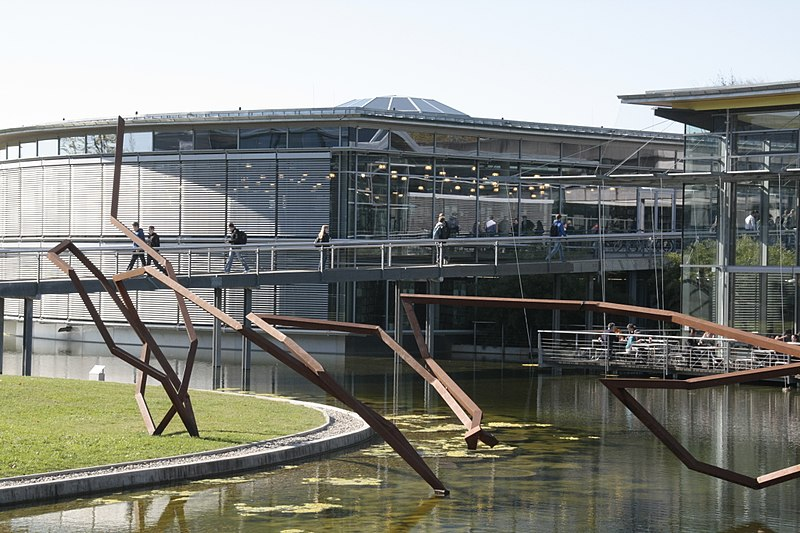
\includegraphics[width=1\textwidth]{images/oth}
	\end{figure}
\end{columns}

\blfootnote{Bild: \href{https://de.wikipedia.org/wiki/Datei:OTH_Regensburg_01.jpg}{https://de.wikipedia.org/wiki/Ostbayerische\_Technische\_Hochschule}}
\end{frame}

%%%%%%%%%%
%
% Problem: Redundante Klimatechnik
%
%%%%%%%%%%
\begin{frame}[fragile]{Problem: Redundante Klimatechnik}
\begin{alertblock}{Redundanz $\neq$ Redundanz}
\end{alertblock}
\begin{itemize}
	\item Zentrale Kälteanlage an der Hochschule
	\item Redundant ausgelegte Kälteanlage
	\item Redundanter Wärmetauscher
	\item Beide an Kälteanlage angeschlossen
	\item Pumpenausfall führte zu Ausfall aller Wärmetauscher
	\item Notabschaltung eines Serverraums nötig
\end{itemize}
\end{frame}

%%%%%%%%%%
%
% Problem: Stromausfälle
%
%%%%%%%%%%
\begin{frame}[fragile]{Problem: Stromausfälle}

\begin{columns}[T,c,onlytextwidth]
	\column{0.6\textwidth}
	\begin{itemize}
		\item Ausfall durch USV gepuffert
		\item Reale Pufferzeit $\neq$ Angegebene Pufferzeit
		\item Längerfristige Pufferung durch Diesel
		\item Regelmäßige Wartung
		\item Immer echte Tests! Regelmäßig 
	\end{itemize}
	\column{0.4\textwidth}
	\begin{figure}
		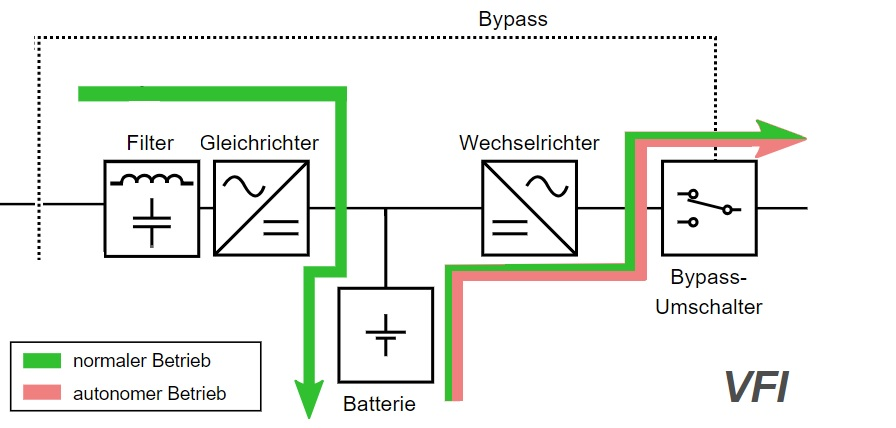
\includegraphics[width=1\textwidth]{images/usv}
	\end{figure}
\end{columns}

\blfootnote{Bild: \href{https://de.wikipedia.org/wiki/Unterbrechungsfreie_Stromversorgung}{https://de.wikipedia.org/wiki/Unterbrechungsfreie\_Stromversorgung}}
\end{frame}

%%%%%%%%%%
%
% Unbeabsichtigte Änderung/Löschung
%
%%%%%%%%%%
\begin{frame}[fragile]{Unbeabsichtigte Änderung/Löschung}
	\begin{itemize}
	\item Unbeabsichtigte Änderungen passieren
	\item Fallen oft Jahre nicht auf
	\item Funktion zur Wiederherstellung an User
	\item Gibt auch Sicherheit
	\item Die Backupfunktion kann ausfallen 
\end{itemize}
\end{frame}

%%%%%%%%%%
%
% Problem: Mehrstufige Backups
%
%%%%%%%%%%
\begin{frame}[fragile]{Problem: Mehrstufige Backups}
	\begin{itemize}
	\item Wiederherstellung von Windows war nicht möglich
	\item Fehler ist erst Monate später aufgefallen
	\item Keine Datensicherung vorhanden
	\item zweite Stufe (LUN-Snapshot)
	\item Wiederherstellung aufwändig aber möglich
\end{itemize}
\end{frame}

%%%%%%%%%%
%
% Problem: Festplattenausfall
%
%%%%%%%%%%
\begin{frame}[fragile]{Problem: Festplattenausfall}
\begin{columns}[T,c,onlytextwidth]
	\column{0.6\textwidth}
	\begin{itemize}
		\item Konfiguration: RAID 60 mit zwei Hot-Spare Platten
		\item Festplattenausfall
		\item Hot-Spare Sicherung: Zweite HDD defekt
		\item Festplattentausch innerhalb von 4 h
		\item Hot-Spare Konfiguration überprüft
	\end{itemize}
	\column{0.4\textwidth}
	\begin{figure}
		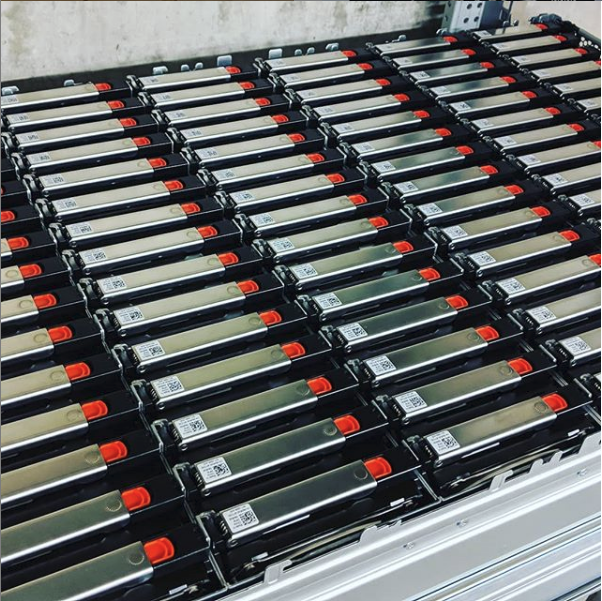
\includegraphics[width=1\textwidth]{images/hdd}
	\end{figure}
\end{columns}
\end{frame}


%%%%%%%%%%
%
% Deduplizierung und Kompression sind deine Freunde
%
%%%%%%%%%%
\begin{frame}[fragile]{Deduplizierung und Kompression sind deine Freunde}
	\begin{itemize}
	\item Deduplizierung: Doppelte Dateien einmal ablegen
	\item Kompression: Dateien komprimieren
	\item Besonders effizient bei Snapshots
	\item Extreme Einsparung möglich
	\item Brutto-Speicherplatz steigt
	\item Beispiel OTH: 45,95 \%
\end{itemize}
\end{frame}

%%%%%%%%%%
%
% Problem: Speicherung über 50 Jahre
%
%%%%%%%%%%
\begin{frame}[fragile]{Problem: Speicherung über 50 Jahre}
	\begin{itemize}
	\item Kein Hersteller garantiert \textgreater 10 Jahre
	\item Migration über Jahre hinweg auf jeweils neues System
	\item Standortunabhängigkeit
	\item Desasterrecovery schwer
	\item Retention Lock muss fortgeführt werden
\end{itemize}
\end{frame}

%%%%%%%%%%
%
% Problem: Fehler entdecken
%
%%%%%%%%%%
\begin{frame}[fragile]{Problem: Fehler entdecken}

\begin{columns}[T,c,onlytextwidth]
	\column{0.6\textwidth}
	\begin{itemize}
	\item Fehler passieren immer
	\item Nur bei Erkennung Reaktion möglich
	\item Schon bei wenig System schnell unübersichtlich
	\item Empfehlung: check\_mk
\end{itemize}
	\column{0.4\textwidth}
	\begin{figure}
		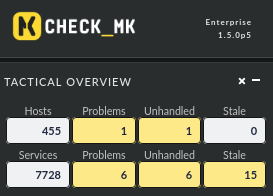
\includegraphics[width=1\textwidth]{images/omd}
	\end{figure}
\end{columns}
\end{frame}


%%%%%%%%%%
%
% Problem: Single Point of Failure
%
%%%%%%%%%%
\begin{frame}[fragile]{Problem: Single Point of Failure}
	\begin{figure}
	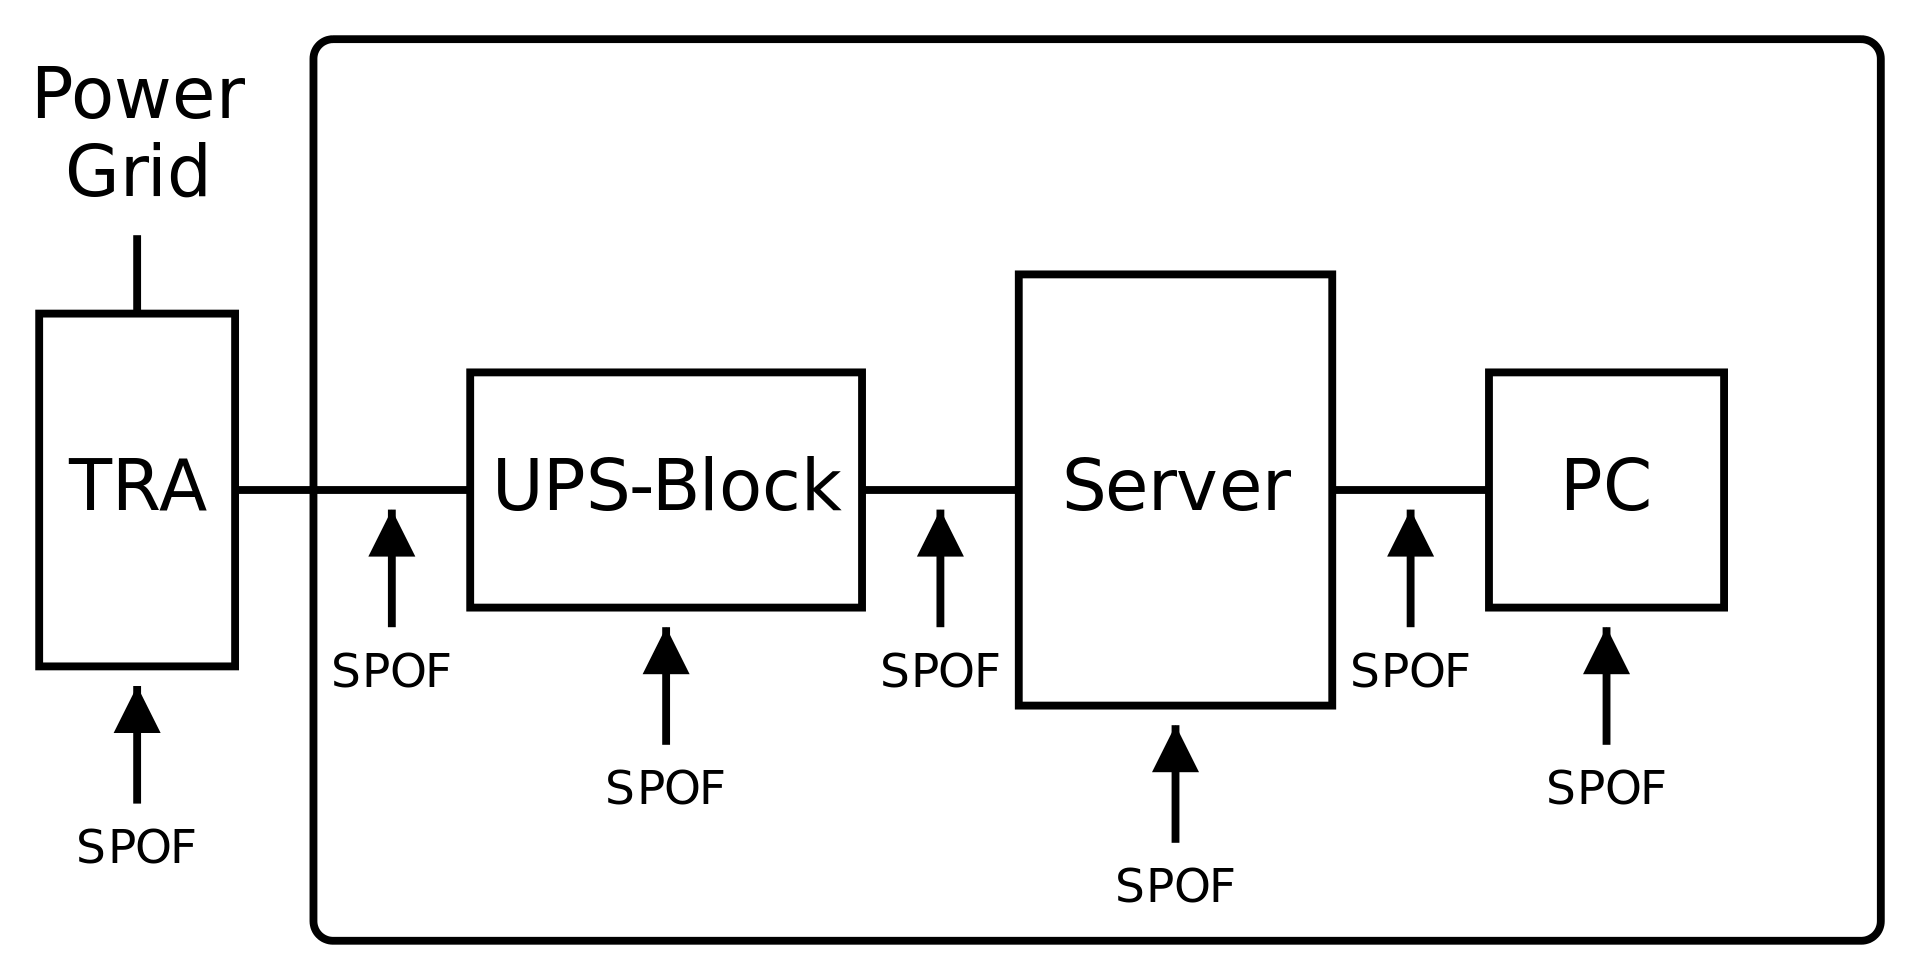
\includegraphics[width=1\textwidth]{images/spof1}
\end{figure}
\blfootnote{Bild: \href{https://de.wikipedia.org/wiki/Single_Point_of_Failure}{https://de.wikipedia.org/wiki/Single\_Point\_of\_Failure}}
\end{frame}

\begin{frame}[fragile]{Problem: Single Point of Failure}
\begin{figure}
	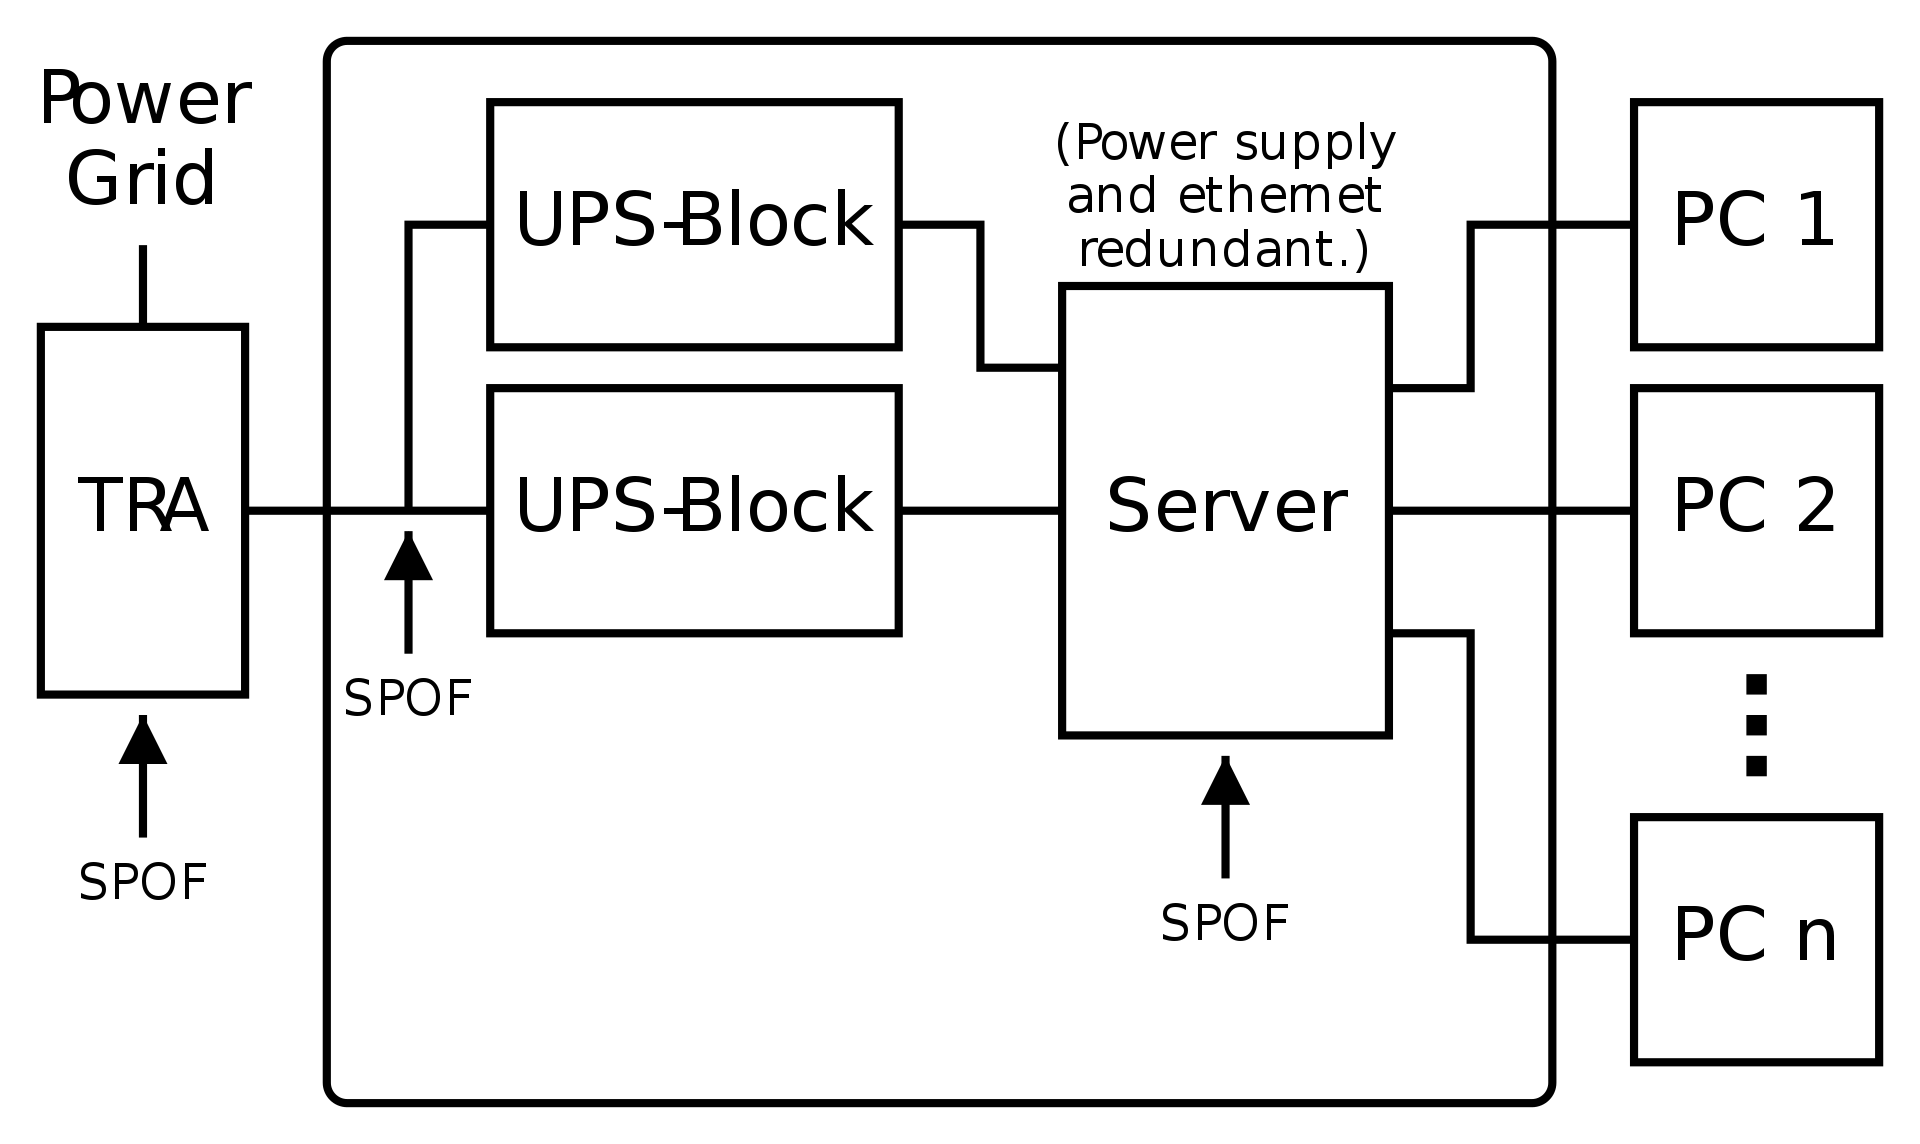
\includegraphics[width=1\textwidth]{images/spof2}
\end{figure}
\blfootnote{Bild: \href{https://de.wikipedia.org/wiki/Single_Point_of_Failure}{https://de.wikipedia.org/wiki/Single\_Point\_of\_Failure}}
\end{frame}

\begin{frame}[fragile]{Problem: Single Point of Failure}
\begin{figure}
	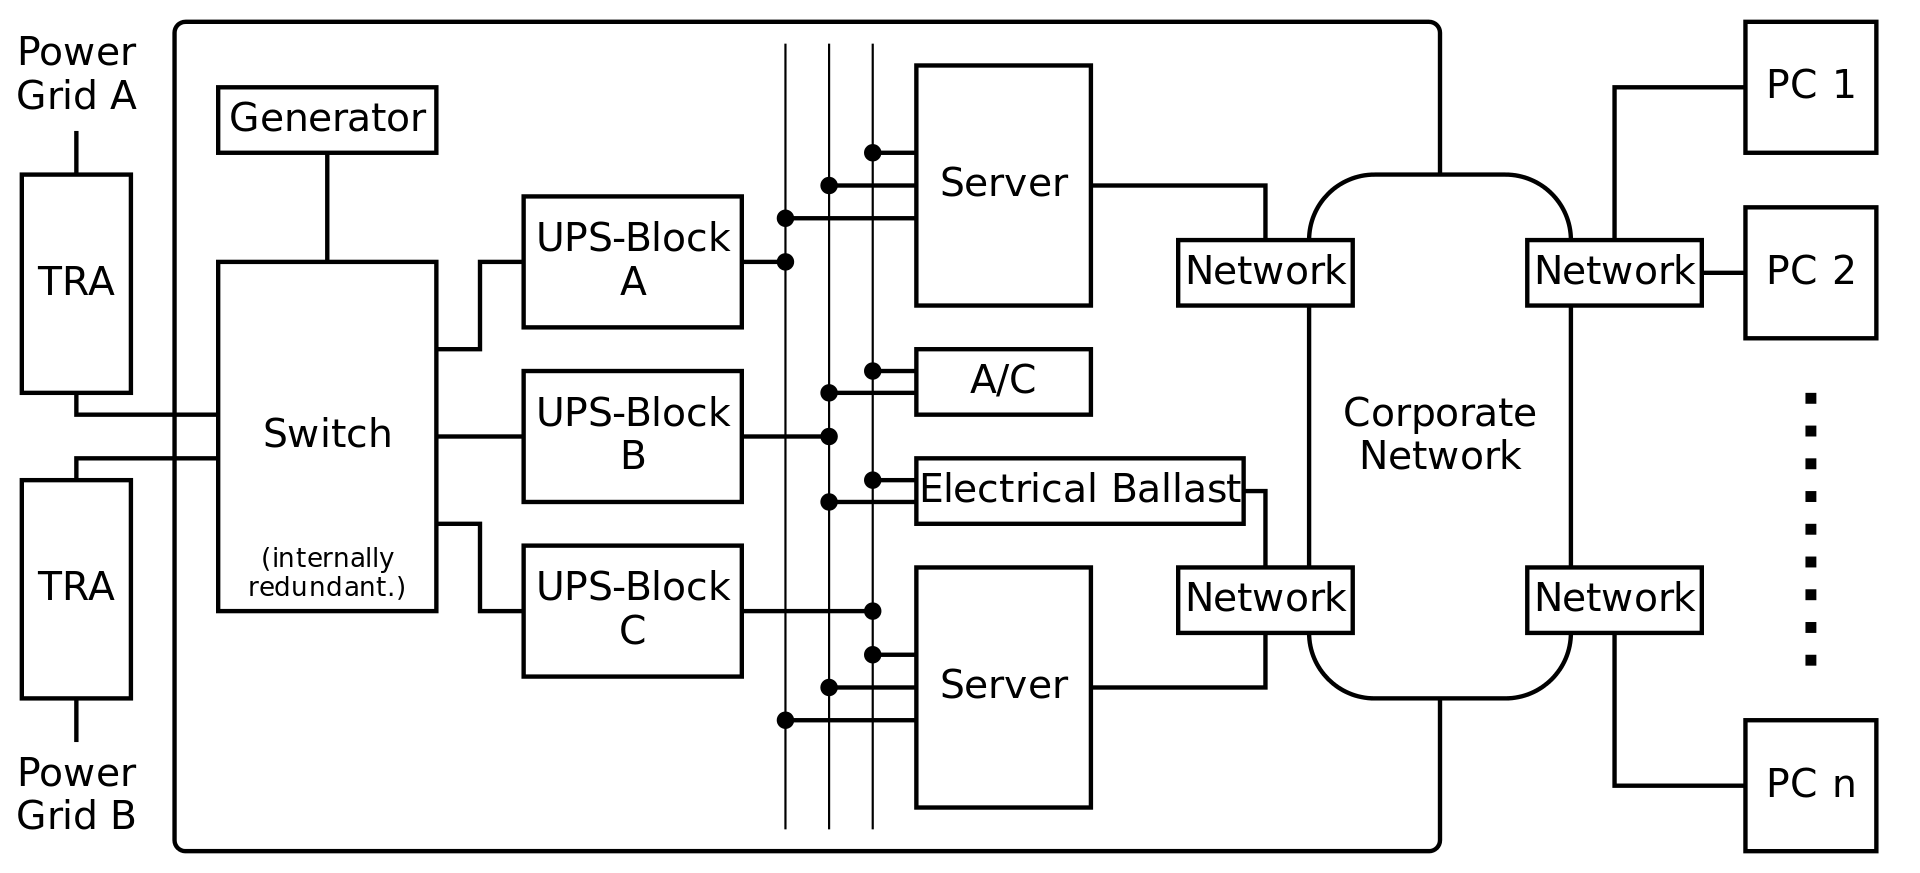
\includegraphics[width=1\textwidth]{images/spof3}
\end{figure}
\blfootnote{Bild: \href{https://de.wikipedia.org/wiki/Single_Point_of_Failure}{https://de.wikipedia.org/wiki/Single\_Point\_of\_Failure}}
\end{frame}

%%%%%%%%%%
%
% Problem: Netzwerkverteilung
%
%%%%%%%%%%
\begin{frame}[fragile]{Problem: Netzwerkverteilung}
	\begin{itemize}
	\item Klimatechnik auch bei Netzwerkknotenpunkten
	\item Ringkonfiguration wegen Bauarbeiten
	\item SPOF zwischen Rechenzentren minimieren
\end{itemize}
\end{frame}

%%%%%%%%%%
%
% Problem: Angriffe
%
%%%%%%%%%%
\begin{frame}[fragile]{Problem: Angriffe}
	\begin{itemize}
		\item Abhärtung der Systeme
		\item Schulung der Mitarbeiter
		\item Anderen Servern sollte nicht vertraut werden
		\item Beispiel: OpenVAS
		\item Beispiel: Logmanagement
		\item Allgemein: Extrem schwer, alle Angriffe abzuhalten
\end{itemize}
\end{frame}

%%%%%%%%%%
%
% Reaktionszeiten
%
%%%%%%%%%%
\begin{frame}[fragile]{Reaktionszeiten}
	\begin{itemize}
	\item Ausfälle passieren!
\item Wie ist die Reaktionszeit?
\item Bei kritischen Systemen: Externer Service
\item Wie schnell kann Ersatz bestellt werden?
\item Eventuell: Vorhalten bestimmter Komponenten
\end{itemize}
\end{frame}

\section{Grundlagen: Verschlüsselung und Signierung}

%%%%%%%%%%
%
% Warum Verschlüsselung?
%
%%%%%%%%%%
\begin{frame}[fragile]{Warum Verschlüsselung?}
	\begin{itemize}
	\item Firmenumfeld und Privat: Immer schützenswerte Daten!
	\item Verschlüsselung schafft vertrauen
	\item Vertrauen unabhängig von einzelnen
	\item Verschlüsselung teilweise gesetzlich gefordert
	\item Am besten: Allgegenwärtig und immer!
	\item Aber: Verschlüsselung auch unbequem
\end{itemize}
\end{frame}

%%%%%%%%%%
%
% Symmetrische Verschlüsselung
%
%%%%%%%%%%
\begin{frame}[fragile]{Symmetrische Verschlüsselung}
\begin{columns}[T,c,onlytextwidth]
	\column{0.6\textwidth}
	\begin{itemize}
		\item Ein gemeinsames Geheimnis
		\item Effiziente Implementierung
		\item Problem des Schlüsselaustausches
		\item Beispiele: AES oder Blowfish 
	\end{itemize}
	\column{0.4\textwidth}
	\begin{figure}
		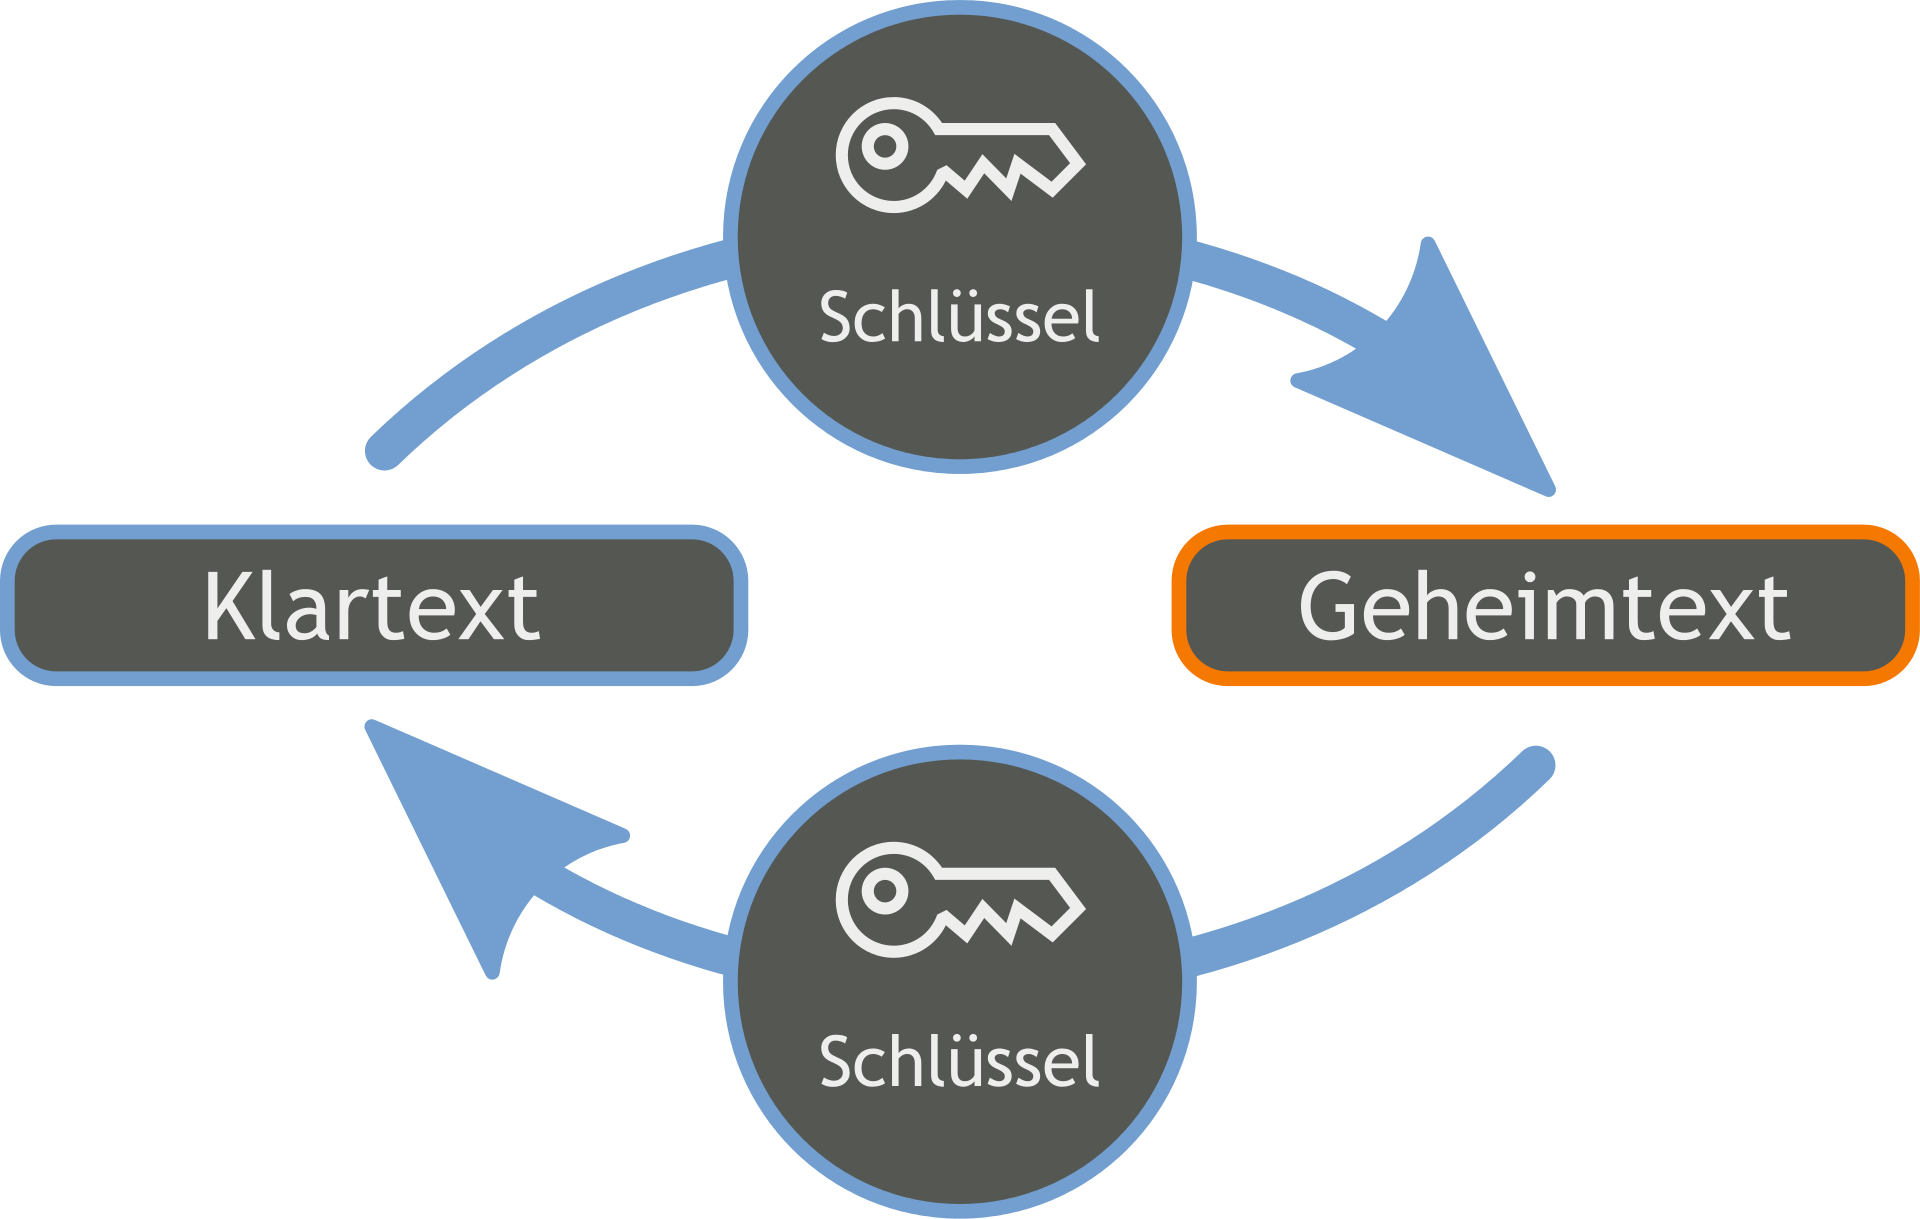
\includegraphics[width=1\textwidth]{images/sym}
	\end{figure}
\end{columns}
\blfootnote{Bild: \href{https://de.wikipedia.org/wiki/Symmetrisches_Kryptosystem}{https://de.wikipedia.org/wiki/Symmetrisches\_Kryptosystem}}
\end{frame}

%%%%%%%%%%
%
% Asymmetrische Verschlüsselung
%
%%%%%%%%%%
\begin{frame}[fragile]{Asymmetrische Verschlüsselung}
\begin{columns}[T,c,onlytextwidth]
	\column{0.6\textwidth}
	\begin{itemize}
		\item Ein Schlüsselpaar
		\item Erster Teil: Nur Verschlüsseln
		\item Zweiter Teil: Nur Entschlüsseln
		\item Key zum Verschlüsseln öffentlich
		\item Key zum Entschlüsseln geheim
		\item Rechenintensiv
		\item Beispiele: RSA, Elliptic Curve Cryptography (ECC)
	\end{itemize}
	\column{0.4\textwidth}
	\begin{figure}
		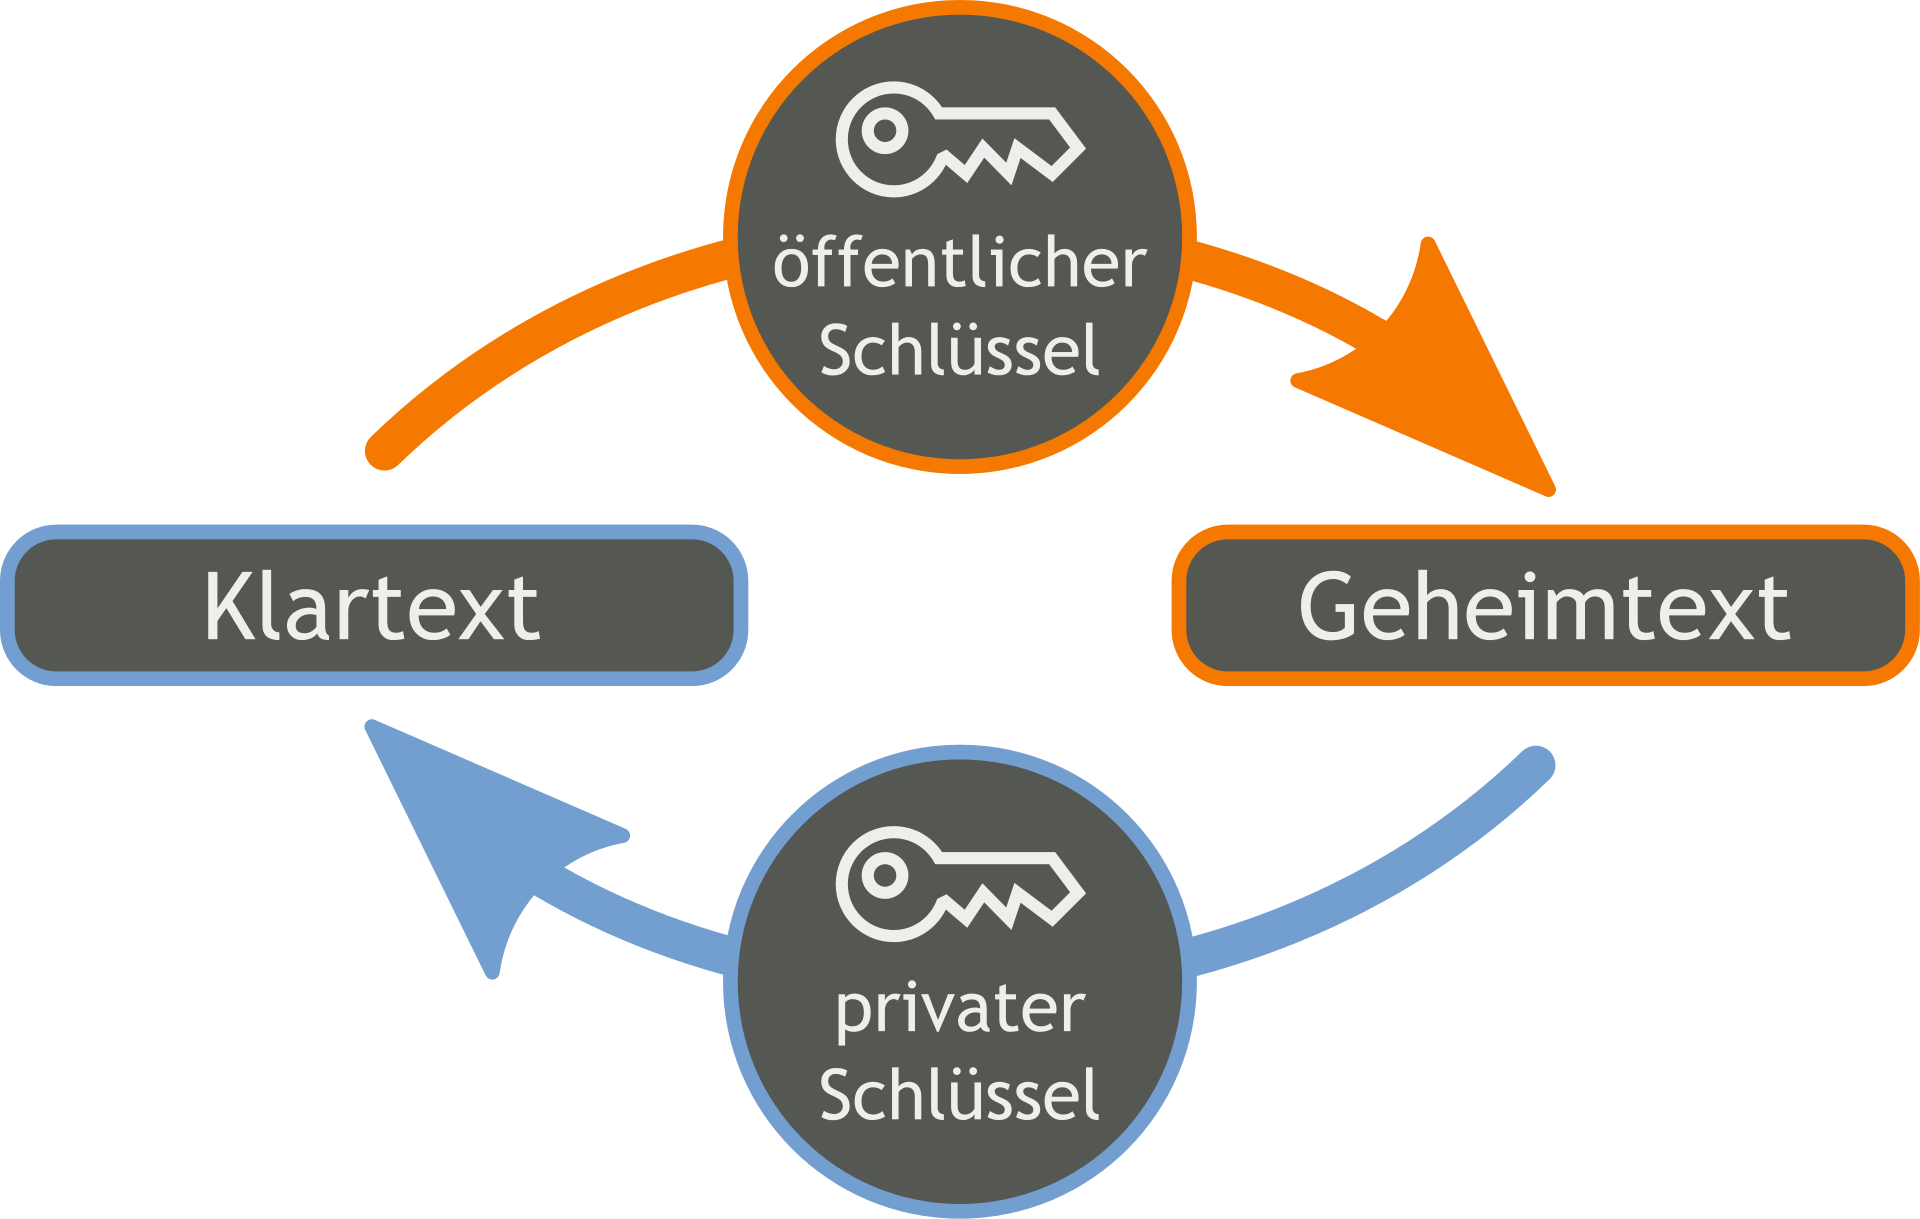
\includegraphics[width=1\textwidth]{images/asym}
	\end{figure}
\end{columns}
\blfootnote{Bild: \href{https://de.wikipedia.org/wiki/Asymmetrisches_Kryptosystem}{https://de.wikipedia.org/wiki/Asymmetrisches\_Kryptosystem}}
\end{frame}

%%%%%%%%%%
%
% Transportverschlüsselung
%
%%%%%%%%%%
\begin{frame}[fragile]{Transportverschlüsselung}
\begin{columns}[T,c,onlytextwidth]
	\column{0.6\textwidth}
	\begin{itemize}
		\item 1. Verschlüsselte Verbindung
		\item 2. Authentizität
		\item Kombination aus Symmetrischer und Asymmetrischer-Verschlüsselung
		\item Zertifikatsketten sorgen für Authentizität
		\item TLS ist nicht gleich TLS
	\end{itemize}
	\column{0.4\textwidth}
	\begin{figure}
		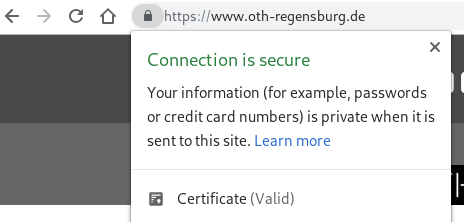
\includegraphics[width=1\textwidth]{images/oth-key}
	\end{figure}
\end{columns}
\end{frame}

%%%%%%%%%%
%
% Festplattenverschlüsselung
%
%%%%%%%%%%
\begin{frame}[fragile]{Festplattenverschlüsselung}
	\begin{itemize}
	\item Extrem wichtig bei mobilen Geräten
	\item Auch wichtig für Cloud-Speicher
	\item Meist AES = Schnelle Implementation
	\item Komplex bei Aufsetzen und starten
	\item Wichtig für Datenschutz bei Diebstahl
\end{itemize}
\end{frame}

%%%%%%%%%%
%
% Signaturalgorithmen
%
%%%%%%%%%%
\begin{frame}[fragile]{Signaturalgorithmen}
	\begin{itemize}
	\item Basiert meist auf Asymmetrischen Kryptographiesystemen
	\item Integrität elektronischer Information gesichert
	\item Zeitstempel kryptographisch gesichert
	\item Wichtig für Compliance
	\item Unverzichtbar bei Revisionssicherheit
\end{itemize}
\end{frame}

%%%%%%%%%%
%
% Email-Verschlüsselung: PGP und S/MIME
%
%%%%%%%%%%
\begin{frame}[fragile]{Email-Verschlüsselung: PGP und S/MIME}
\begin{columns}[T,c,onlytextwidth]
	\column{0.5\textwidth}
\begin{itemize}
	\item Email nur Transportverschlüsselt
\item Ansonsten: Postkarte
\item Absender kann ohne weiteres gefälscht werden
\item Mögliche Methoden: \\PGP und S/MIME
\end{itemize}
\column{0.5\textwidth}
\begin{figure}
	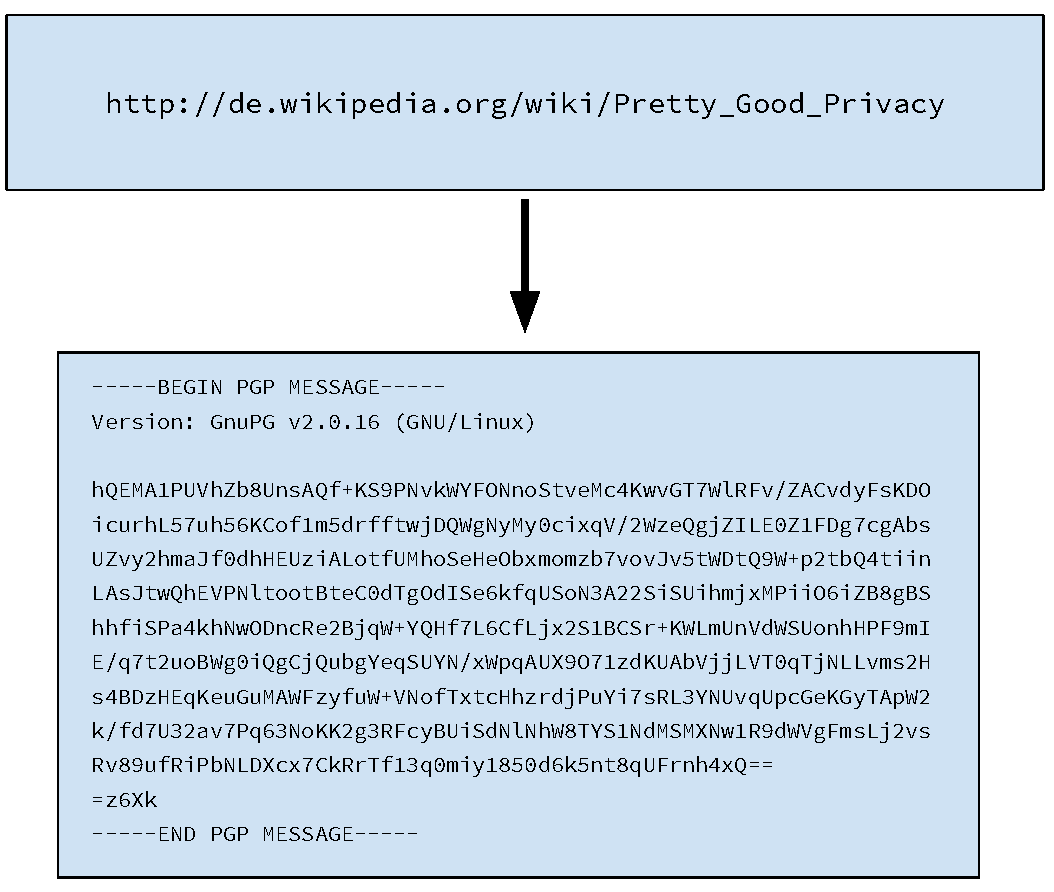
\includegraphics[width=1\textwidth]{images/pgp}
\end{figure}
\end{columns}
\end{frame}

\section{Verschlüsselung und Signierung in der Praxis}

%%%%%%%%%%
%
% TLS für Websites
%
%%%%%%%%%%
\begin{frame}[fragile]{TLS für Websites}
\begin{figure}
	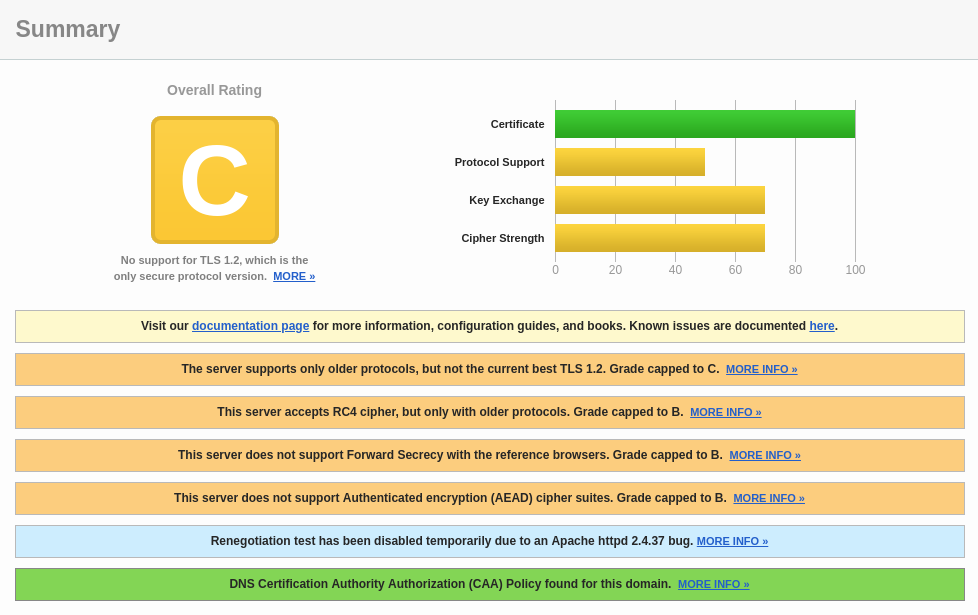
\includegraphics[width=1\textwidth]{images/not-secure1}
\end{figure}
\blfootnote{Bild: Screenshot -  \href{https://www.ssllabs.com/ssltest}{https://www.ssllabs.com/ssltest}}
\end{frame}

\begin{frame}[fragile]{TLS für Websites}
\begin{figure}
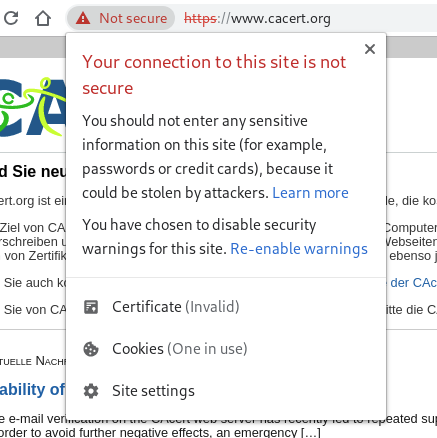
\includegraphics[width=0.5\textwidth]{images/not-secure2}
\end{figure}
\blfootnote{Bild: Screenshot Chrome}}
\end{frame}

\begin{frame}[fragile]{TLS für Websites}
\begin{figure}
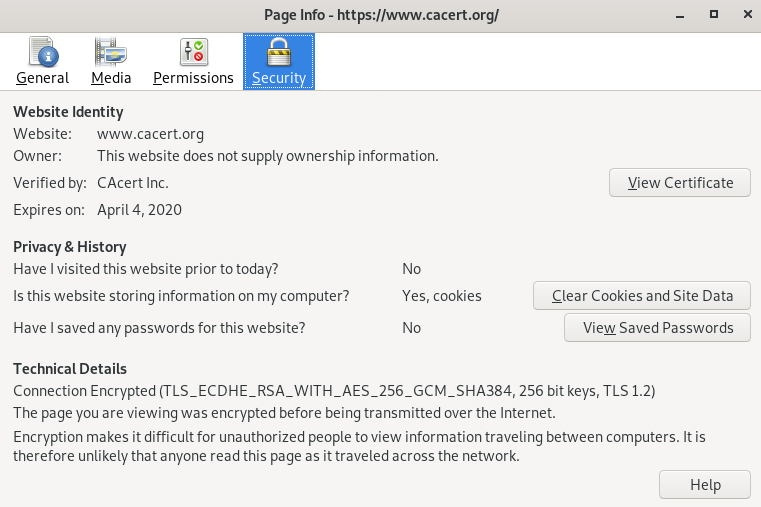
\includegraphics[width=0.9\textwidth]{images/not-secure3}
\end{figure}
\blfootnote{Bild: Screenshot Firefox}}
\end{frame}

\begin{frame}[fragile]{TLS für Websites}
\begin{alertblock}{Tipps}
\end{alertblock}
	\begin{itemize}
	\item Nogo: Website ohne TLS
	\item TLS ist kein Hexenwerk mehr
	\item Kostenlose Zertifikate: letsencrypt.org
	\item Gute Verschlüsselung: cipherli.st
	\item Stichwort: TLS 1.3 vs. eTLS
\end{itemize}
\end{frame}

%%%%%%%%%%
%
% Email-Verschlüsselung in der Praxis
%
%%%%%%%%%%
\begin{frame}[fragile]{Email-Verschlüsselung in der Praxis}
\begin{columns}[T,c,onlytextwidth]
	\column{0.6\textwidth}
	\begin{itemize}
		\item pEp: Pretty Easy Privacy
		\item Standard Verschlüsselugnsverfahren
		\item Einfach umgesetzt
		\item Outlook, Thunderbird, Android, iOS
		\item www.pep.security
	\end{itemize}
	\column{0.4\textwidth}
	\begin{figure}
		
\includegraphics[width=0.9\textwidth]{images/pep}
	\end{figure}
\end{columns}
\blfootnote{Bild: \href{https://de.wikipedia.org/wiki/Pretty_Easy_privacy}{https://de.wikipedia.org/wiki/Pretty\_Easy\_privacy}}
\end{frame}

%%%%%%%%%%
%
% Ausflug: Whatsapp und Co
%
%%%%%%%%%%
\begin{frame}[fragile]{Ausflug: Whatsapp und Co}
	\begin{itemize}
	\item Messenger praktisch für schnelle Kommunikation
	\item WhatsApp Ende-zu-Ende verschlüsselt
	\item Verwendet Signal-Protokoll
	\item Metadaten unverschlüsselt
	\item Backups unverschlüsselt
	\item Bessere Alternativen möglich
	\item Beispiel: Signal
\end{itemize}
\end{frame}

\section{Zusammenfassung}

%%%%%%%%%%
%
% Zusammenfassung
%
%%%%%%%%%%
\begin{frame}[fragile]{Zusammenfassung}
	\begin{itemize}
	\item Backups sind kein einfaches Thema
	\item Verschlüsselung noch weniger
	\item Viel zu beachten
	\item Aber: Einfache Backups besser als Keine
	\item Gute Vorbereitung Hilft im Fehlerfall
\end{itemize}
\end{frame}

%%%%%%%%%%
%
% Kontakt
%
%%%%%%%%%%
\begin{frame}[fragile]{Kontakt}
	\begin{exampleblock}{Timo Schindler}
		timo.schindler@oth-regensburg.de
	\end{exampleblock}
\end{frame}

\end{document}
